%%%%%%%%%%%%%%%%%%%%%%%%%%%%%%%%%%%%%%%%%
% Wenneker Article
% LaTeX Template
% Version 2.0 (28/2/17)
%
% This template was downloaded from:
% http://www.LaTeXTemplates.com
%
% Authors:
% Vel (vel@LaTeXTemplates.com)
% Frits Wenneker
%
% License:
% CC BY-NC-SA 3.0 (http://creativecommons.org/licenses/by-nc-sa/3.0/)
%
%%%%%%%%%%%%%%%%%%%%%%%%%%%%%%%%%%%%%%%%%

%----------------------------------------------------------------------------------------
%	PACKAGES AND OTHER DOCUMENT CONFIGURATIONS
%----------------------------------------------------------------------------------------


%\documentclass[10pt, a4paper, twocolumn]{article}
\documentclass[10pt, a4paper]{article}% 10pt font size (11 and 12 also possible), A4 paper (letterpaper for US letter) and two column layout (remove for one column)

%%%%%%%%%%%%%%%%%%%%%%%%%%%%%%%%%%%%%%%%%
% Wenneker Article
% Structure Specification File
% Version 1.0 (28/2/17)
%
% This file originates from:
% http://www.LaTeXTemplates.com
%
% Authors:
% Frits Wenneker
% Vel (vel@LaTeXTemplates.com)
%
% License:
% CC BY-NC-SA 3.0 (http://creativecommons.org/licenses/by-nc-sa/3.0/)
%
%%%%%%%%%%%%%%%%%%%%%%%%%%%%%%%%%%%%%%%%%

%----------------------------------------------------------------------------------------
%	PACKAGES AND OTHER DOCUMENT CONFIGURATIONS
%----------------------------------------------------------------------------------------

\usepackage[spanish]{babel} % English language hyphenation

\usepackage{microtype} % Better typography

\usepackage{amsmath,amsfonts,amsthm} % Math packages for equations

%\usepackage[svgnames]{xcolor} % Enabling colors by their 'svgnames'

% \usepackage[hang, small, labelfont=bf, up, textfont=it]{caption} % Custom captions under/above tables and figures

\usepackage{booktabs} % Horizontal rules in tables

\usepackage{lastpage} % Used to determine the number of pages in the document (for "Page X of Total")

% \usepackage{graphicx} % Required for adding images

\usepackage{enumitem} % Required for customising lists
\setlist{noitemsep} % Remove spacing between bullet/numbered list elements

\usepackage{sectsty} % Enables custom section titles
\allsectionsfont{\usefont{OT1}{phv}{b}{n}} % Change the font of all section commands (Helvetica)

\usepackage{hyperref} % Required for hyperlinks
\hypersetup{hidelinks,colorlinks,breaklinks=true,urlcolor=Blue,citecolor=Green,linkcolor=DarkBlue,bookmarksopen=false,pdftitle={Title},pdfauthor={Author}}

\usepackage{lipsum} % Required to insert dummy text. To be removed otherwise
\usepackage{listings} % Para la parte de los keywords

%----------------------------------------------------------------------------------------
%	MARGINS AND SPACING
%----------------------------------------------------------------------------------------

% \usepackage{geometry} % Required for adjusting page dimensions

% \geometry{
% 	top=1cm, % Top margin
% 	bottom=1.5cm, % Bottom margin
% 	left=2cm, % Left margin
% 	right=2cm, % Right margin
% 	includehead, % Include space for a header
% 	includefoot, % Include space for a footer
% 	%showframe, % Uncomment to show how the type block is set on the page
% }

% \setlength{\columnsep}{7mm} % Column separation width

%----------------------------------------------------------------------------------------
%	FONTS
%----------------------------------------------------------------------------------------

\usepackage[T1]{fontenc} % Output font encoding for international characters
\usepackage[utf8]{inputenc} % Required for inputting international characters

\usepackage{XCharter} % Use the XCharter font

%----------------------------------------------------------------------------------------
%	HEADERS AND FOOTERS
%----------------------------------------------------------------------------------------

% \usepackage{fancyhdr} % Needed to define custom headers/footers
% \pagestyle{fancy} % Enables the custom headers/footers

% \renewcommand{\headrulewidth}{0.0pt} % No header rule
% \renewcommand{\footrulewidth}{0.4pt} % Thin footer rule

% \renewcommand{\sectionmark}[1]{\markboth{#1}{}} % Removes the section number from the header when \leftmark is used

%\nouppercase\leftmark % Add this to one of the lines below if you want a section title in the header/footer

% % Headers
% \lhead{} % Left header
% \chead{\textit{\thetitle}} % Center header - currently printing the article title
% \rhead{} % Right header

% % Footers
% \lfoot{} % Left footer
% \cfoot{} % Center footer
% \rfoot{\footnotesize Page \thepage\ of \pageref{LastPage}} % Right footer, "Page 1 of 2"

%\fancypagestyle{firstpage}{ % Page style for the first page with the title
% 	\fancyhf{}
% 	\renewcommand{\footrulewidth}{0pt} % Suppress footer rule
% }

%----------------------------------------------------------------------------------------
%	TITLE SECTION
%----------------------------------------------------------------------------------------

%\newcommand{\keywordname}{Keywords} % Defines the keywords heading name
\newcommand{\keywordname}{Keywords: \color{DarkBlue}} % Defines the keywords heading name

\newcommand{\authorstyle}[1]{{\large\usefont{OT1}{phv}{b}{n}\color{DarkRed}#1}} % Authors style (Helvetica)

\newcommand{\institution}[1]{{\footnotesize\usefont{OT1}{phv}{m}{sl}\color{Black}#1}} % Institutions style (Helvetica)

\usepackage{titling} % Allows custom title configuration

\newcommand{\HorRule}{\color{DarkGoldenrod}\rule{\linewidth}{1pt}} % Defines the gold horizontal rule around the title

\pretitle{
	\vspace{-55pt} % Move the entire title section up
	\HorRule\vspace{10pt} % Horizontal rule before the title
	\fontsize{24}{30}\usefont{OT1}{phv}{b}{n}\selectfont % Helvetica
	\color{DarkRed} % Text colour for the title and author(s)
}

\posttitle{\par\vskip 15pt} % Whitespace under the title

\preauthor{} % Anything that will appear before \author is printed

\postauthor{ % Anything that will appear after \author is printed
	\vspace{10pt} % Space before the rule
	\par\HorRule % Horizontal rule after the title
	\vspace{-45pt} % Space after the title section
}

%----------------------------------------------------------------------------------------
%	ABSTRACT
%----------------------------------------------------------------------------------------

\usepackage{lettrine} % Package to accentuate the first letter of the text (lettrine)
\usepackage{fix-cm}	% Fixes the height of the lettrine

\newcommand{\initial}[1]{ % Defines the command and style for the lettrine
	\lettrine[lines=1,findent=4pt,nindent=0pt]{% Lettrine takes up 3 lines, the text to the right of it is indented 4pt and further indenting of lines 2+ is stopped
		\color{DarkGoldenrod}% Lettrine colour
		{#1}% The letter
	}{}%
}

\usepackage{xstring} % Required for string manipulation

\newcommand{\lettrineabstract}[1]{
	\StrLeft{#1}{1}[\firstletter] % Capture the first letter of the abstract for the lettrine
	\initial{\firstletter}\textbf{\StrGobbleLeft{#1}{1}} % Print the abstract with the first letter as a lettrine and the rest in bold
}

%----------------------------------------------------------------------------------------
%	BIBLIOGRAPHY
%----------------------------------------------------------------------------------------

\usepackage[backend=bibtex,style=authoryear,natbib=true]{biblatex} % Use the bibtex backend with the authoryear citation style (which resembles APA)

\addbibresource{example.bib} % The filename of the bibliography

\usepackage[autostyle=true]{csquotes} % Required to generate language-dependent quotes in the bibliography
 % Specifies the document structure and loads requires packages
\usepackage[sc]{mathpazo} % Use the Palatino font
\usepackage[T1]{fontenc} % Use 8-bit encoding that has 256 glyphs
\linespread{1.05} % Line spacing - Palatino needs more space between lines
%\usepackage{microtype} % Slightly tweak font spacing for aesthetics

\usepackage[twoside,width=16cm,height=24cm,left=3cm]{geometry}
%\usepackage[hmarginratio=1:1,top=20mm,width=19cm,height=23cm,columnsep=15pt]{geometry} % Document margins
\usepackage{multicol} % Used for the two-column layout of the document
\usepackage[hang, small,labelfont=bf,up,textfont=it,up]{caption} % Custom captions under/above floats in tables or figures
\usepackage{booktabs} % Horizontal rules in tables
\usepackage{float} % Required for tables and figures in the multi-column environment - they need to be placed in specific locations with the [H] (e.g. \begin{table}[H])
\usepackage{hyperref} % For hyperlinks in the PDF

%----------- Agregados para el caso de ustedes -------------------------------
\usepackage[spanish]{babel}% idioma castellano
\usepackage[utf8]{inputenc}% esto es para poder poner los tildes directamente. Puede que cambie de versión a versión de sistema operativos (más información en http://www.aq.upm.es/Departamentos/Fisica/agmartin/webpublico/latex/FAQ-CervanTeX/FAQ-CervanTeX-6.html )
\usepackage{graphicx} % para insertar figuras
\usepackage{subfigure} % para insertar figuras dentro de figuras
\usepackage{times} % plataforma
\usepackage{amsmath} % --para ecuaciones y algunos símbolos 
% ---------------------- -----------------------------------------------------

\usepackage{lettrine} % The lettrine is the first enlarged letter at the beginning of the text
%\usepackage{paralist} % Used for the compactitem environment which makes bullet points with less space between them


\usepackage{abstract} % Allows abstract customization
\renewcommand{\abstractnamefont}{\normalfont\bfseries} % Set the "Abstract" text to bold
\renewcommand{\abstracttextfont}{\normalfont\itshape} % Set the abstract itself to small italic text
\addto\captionsspanish{ % Modifica algunos nombres cambiandolos por los definidos a continuacion
        \def\contentsname{\'Indice}%
        \def\bibname{Referencias}%
        \def\tablename{Tabla}%
        \def\abstractname{Resumen}
        }
\usepackage[usenames,dvipsnames,svgnames,table]{xcolor}
%\usepackage{natbib}
%\usepackage[usenames]{color}
\usepackage{graphicx}
\usepackage[spanish]{babel}
\usepackage{amsmath}
\usepackage{float}
\usepackage{dsfont}
\usepackage{textcomp}
\usepackage{soul}
\usepackage{fancyhdr}
\usepackage{titlesec} % Allows customization of titles
\usepackage{fancyhdr} % Headers and footers
\usepackage[spanish]{babel}
\usepackage{amsmath}
%\usepackage{hyperref}


\pagestyle{fancy} % All pages have headers and footers
 \fancyhead{} % Blank out the default header
 \fancyfoot{} % Blank out the default footer
\fancyhead[C]{Laboratorio  $\bullet$ $\today$ } % Custom header text
\fancyfoot[RO,LE]{\thepage} % Custom footer text


 %incluye los paquetes usados mas comunes 

%----------------------------------------------------------------------------------------
%	INFORMACION DEL ARTICULO
%----------------------------------------------------------------------------------------
\title{\centering{Estudio y caracterización de modos transversales electromagnéticos y cavidades de oscilación de un láser Nd:YAG}} % Titulo del Informe

\author{
	\authorstyle{Lucía Evangelista Gallo \textsuperscript{1,1}}
	\authorstyle{Leandro Ariel Pezzente\textsuperscript{1,1}} % Authors
	\newline\newline % Space before institutions
	\textsuperscript{1}\institution{Facultad de Ciencias Exactas y Naturales}\\ % Institution 1
	\textsuperscript{1}\institution{Universidad Nacional de Buenos Aires, Buenos Aires, Argentina}\\ % Institution 1
	\keywordname{Laser --- Nd:YAG --- Modos Transversales --- Cavidades de Oscilación } % Keywords - if you don't want any simply remove all the text between the curly brackets
}

\date{} % Add a date here if you would like one to appear underneath the title block, use \today for the current date, leave empty for no date

%----------------------------------------------------------------------------------------

\begin{document}
\maketitle % Print the title
\thispagestyle{fancy} % All pages have headers and footers
%\thispagestyle{firstpage} % Apply the page style for the first page (no headers and footers)

%----------------------------------------------------------------------------------------
%	ABSTRACT
%----------------------------------------------------------------------------------------

\begin{abstract}
%\lettrineabstract{ 
En este experimento se busca estudiar el comportamiento de la cavidad resonante de un láser de Nd:YAG. Se procede primero a determinar las condiciones de alineación bajo las cuales un espejo dieléctrico de 98\% permite la aparición de modos resonantes en una cavidad lineal , así como también se estudian las características de la potencia óptica emitida por el láser de Nd:YAG tanto en cavidades lineales como en cavidades en V. Finalmente, se analizan los distribución espacial de los diferentes modos transversales electromagnéticos emitidos por el laser  
%}
\end{abstract}
\begin{multicols}{2} % Two-column layout throughout the main article text
%----------------------------------------------------------------------------------------
%	ARTICLE CONTENTS
%----------------------------------------------------------------------------------------
\tableofcontents % Print the contents section

\section{Introducción}
% \addcontentsline{toc}{section}{Introduccion} % Adds this section to the table of contents

Un láser es un dispositivo que permite la amplificación de radiación electromagnética mediante un proceso físico conocido como emisión estimulada o inducida. Estos instrumentos están compuestos por un mecanismo de bombeo, un medio amplificador y un medio de realimentación. En los experimentos realizados, se utilizó un diodo láser como mecanismo de bombeo y una barra de Nd:YAG como medio amplificador. Para el caso de luz, una cavidad resonante (el medio de realimentación) consiste en un arreglo de espejos tal que la luz recorre el mismo camino óptico varias veces. Uno de esos espejos debe tener reflectividad menor al 100\% para permitir la salida de un haz (\textcolor{DarkBlue}{manteniendo a la vez un valor alto del Q de la cavidad}). Se logran distintas cavidades modificando las distancias y los radios de curvatura de los espejos. Dado que se buscaba un haz continuo, se diseñó una cavidad estable, es decir, un recinto donde, dados dos espejos de radios R$_1$ y R$_2$ separados por una distancia $d$, se cumple la siguiente relación:
\begin{equation}
    0 \leq g_1 g_2 \leq 1,
\end{equation}
con $g_i = 1 - d/R_i$. Es importante tener en cuenta que, para que el dispositivo emita luz, las dimensiones de la cavidad deben ser proporcionales (\textcolor{DarkBlue}{un numero entero de veces}) a la longitud de onda de emisión, que en este caso era 1064nm.

Las características más distintivas de los láseres son que la luz emitida por éstos es cuasi-monocromática (ancho de linea espectral pequeño), coherente (diferentes puntos del campo eléctrico oscilan con la misma diferencia de fase), y altamente colimada (baja divergencia del haz).


Uno de los objetivos de este trabajo fue visualizar distintos modos TEM$_{pq}$ (modo transverso electromagnético de orden pq). Dadas las dimensiones de la barra YAG y de los espejos (que no tienen radio infinito), no se pueden formar ondas estacionarias planas dentro de la cavidad resonante. Para el caso de cavidades resonantes sin paredes, como las del láser en cuestión, las soluciones estacionarias son estos modos TEM$_{pq}$. Los números pq son el orden de los polinomios de Hermite(\textcolor{DarkBlue}{-Gauss}) presentes en la parte analítica de la solución (\textcolor{DarkBlue}{Lo cual es un resultado directo de la naturaleza cuantica del campo electromagnetico \texttt{https : // www . sciencedirect . com/science/article /pii/S0143816697000031} }). El modo más bajo es el 00, que presenta un perfil de intensidad gaussiano. Modos <<superiores>> son combinaciones de polinomios de Hermite(\textcolor{DarkBlue}{-Gauss}) en los ejes $x$ e $y$, y los números pq indican la cantidad de ceros en la (\textcolor{DarkBlue}{el perfil de })intensidad (\textcolor{DarkBlue}{del campo de radiacion electromagnetica}), en cada dirección[1].

Luego de visualizar los modos TEM, se buscó generar segunda armónica. Este es un fenómeno de óptica no lineal que consiste en producir un haz láser con la mitad de la longitud de onda original. Así, de un haz infrarrojo ($\lambda$ = 1064nm), se pudo obtener uno verde ($\lambda$ = 532nm)[2].





%%%%%%%%%%%%%%%%%%%%%%%%%%%%%%%%%%%%%%%%%%%%

\iffalse
El láser es un dispositivo que permite la amplificación de radiación electromagnética mediante un proceso físico conocido como emisión estimulada o inducida. Este proceso permite la amplificación de señales lumínicas generadas por otros medios. El mecanismo que genera dichas señales lumínicas se denominada mecanismo de bombeo, y los procesos para generarlo son diversos y pueden ir desde descargas eléctricas en medios gaseoso hasta el uso de otros laseres en la excitación fluorescente de medios orgánicos como colorantes. Esto es necesario para excitar las transiciones electrónicas en el medio en el que se produce la emisión estimulada, denominado medio activo,debido a que se debe entregar energía al medio activo de manera constante para que pueda mantenerse la emisión estimulada.(\textcolor{DarkBlue}{ DANGER WILL ROBINSON DANGER DANGER DANGER!!! No esta muy bien explicado esto, parece una logica circular}) Por ultimo, se necesita de un mecanismo de realimentación a fin de inducir las transiciones electrónicas que producen la amplificación de la radiación electromagnética. El mecanismo de retroalimentación se logra mediante una cavidad resonante que usualmente consiste en dos o mas espejos de alta reflectividad alineados de tal manera de se favorezca la la reinyeccion de la luz emitida en el sentido del eje de la cavidad por el medio activo excitado al mismo medio. Los espejos entonces actúan como un multiplicador de la longitud de onda del material. El mecanismo de retroalimentación es indispensable porque para que la el láser emita, el proceso de bombeo no debe solamente excitar el medio activo, sino que que también debe lograr la condición de población de inversión en la cual hay mas electrones del medio activo en estados excitados de alta energía que en estados de baja energía.
Otro aspecto importante por el cual es crucial la correcta alineación de los espejos en la cavidad, es que , puesto que como el resonador debe sustentar ondas estacionarias de luz, es decir, se debe mantener una configuración estable del campo de radiación.
\newline
Las características mas distintivas de los laseres son que la luz emitida por estos es cuasi-monocromática ( ancho de linea espectral pequeño ), coherente ( diferentes puntos del campo electrico oscilan con la misma diferencia de fase ) y altamente colimada ( baja divergencia del haz ).

\subsection{Condiciones de estabilidad de una cavidad láser }
Se define un resonador óptico o cavidad como el arreglo de componentes ópticos que permite que un haz de luz circule dentro del láser. Para un resonador óptico dado en un láser se tienen modos de oscilación que dependen son o bien dependientes de la frecuencia del haz o bien dependientes de la distribución espacial del haz. Estos últimos modos se denominan modos transversales electromagnéticos, y son una consecuencia del hecho de el haz de luz no es una onda plana sino que posee una distribución espacial finita. Por lo general, un haz láser emitido por una cavidad resonante es una combinación de varios modos de oscilación. Esto es importante al analizar las perdidas por difracción las cuales son mas altas para modos transversales de mayor orden y afectan mas seriamente a la calidad del haz.(\textcolor{DarkBlue}{Lo de definir que es un modo TEM y un perfil gaussiano lo dejo para mas adelante}) Además un resonador óptico puede ser estable o inestable , aquí el termino estabilidad esencialmente significa que cualquier rayo de luz inyectado en el sistema inicialmente con algún ángulo y apartamiento de la posición transversal respecto del eje óptico se mantendrá dentro del sistema durante muchos cada viajes cerrados. Para los resonadores inestables, en cambio, hay rayos que pueden exhibir un incremento ilimitado de su posición transversal, eventualmente divergiendo y abandonando el sistema óptico. La estabilidad de un resonador depende de la disposición particular de los componentes de la cavidad, especialmente de la alineación de los componentes ópticos, la curvatura de las superficies reflectantes, la reflectividad de las superficies y la distancia entre dichos componentes. Si bien la mayoría de los laseres están basados en resonadores estables, los resonadores inestables también presentan ciertas ventajas, como ser un menor nivel de sensibilidad al alineamiento de los componentes,características deseables particularmente en el diseño de laseres con una alta eficiencia y potencia de salida. Sin embargo, los resonadores inestables tienden a tener distribuciones mas complicadas de modos transversales electromagnéticos.
\newline
\textcolor{DarkBlue}{Placeholder para grafico de cavidades estables e inestables}
\newline
El tipos de cavidad estable mas frecuentemente utilizadas es la cavidad conformada por dos espejos separados a una distancia d. Para el caso de dos espejos planos paralelos , esta cavidad se conoce como resonador de Fabry-Perot y para el caso con dos espejos esféricos ({\textcolor{DarkBlue}{¿curvos?}}) se tienen diversos tipos configuraciones para el resonador optico como los resonadores concéntricos y los resonadores confocales . Para el caso de resonadores de Fabry-Perot la condición de estabilidad se obtiene de imponer que la distancia d entre los espejos, esto es, el largo de la cavidad, sea a primera aproximación de los modos, igual a un numero entero de medias longitudes de onda, ${ d = n \frac{\lambda}{2} }$ donde ${\lambda}$ es la longitud de onda del haz y n es un numero entero.Para el caso de dos espejos esféricos, es de particular interés el resonador de tipo confocal. Este resonador consiste de dos espejos de diferente radio de curvatura R1 y R2 separados a una distancia focales de ambos espejos caigan en el mismo punto. Esta configuración tiene la ventaja es independiente de la dirección en la que viajen los haces de luz. Se tendrá para este caso una cavidad resonante estable si se cumple la condición : 

\begin{equation}
    0 \leq g_1 \cdot g_2 \leq 1
\end{equation}

donde se ha definido ${g_{1,2} = 1 - \frac{d}{R_{1,2}}}$ considerando que los espejos convergente tienen radio de curvatura positivo.

\fi

\section{Desarrollo experimental}
La primera parte del experimento consistió en armar una cavidad estable y medir cómo afectaba la variación de corriente y de distancia a la potencia de salida del láser y del diodo de bombeo. Para configurar la cavidad, se utilizó un láser auxiliar de He--Ne (Melles Griot 05-LHR-111, $\lambda$ = 632.8 nm ), dos espejos de plata (New Focus 5151/vis, 99.99\% de reflectividad) y un espejo plano con 98\% de reflectividad (el espejo que <<cierra>> la cavidad). Inicialmente se colocaron los espejos de Ag como muestra la Fig. \ref{cavestable}; el primero se encontraba a una distancia horizontal de $(148.5 \pm 0.1)$cm del láser de He--Ne, el segundo a $(169.5 \pm 0.1)$cm del medio óptico (también en la misma línea) y entre ambos espejos había una distancia diagonal de $(155.3 \pm 0.1)$cm. Los espejos estaban montados en posicionadores angulares que habilitaban todos los grados de libertad necesarios para alinearlos. Se comenzó alineando las reflexiones en los espejos de Ag. Una vez logrado, se colocó el espejo dieléctrico plano (R = 50cm, HR @ 1064nm, $\phi$1") a una distancia de $(4.9 \pm 0.1)$cm de la barrita YAG y se repitió el proceso de alineación. Luego, se alimentó el diodo láser con una corriente de 2.3A aproximadamente y se utilizó una tarjeta infrarroja (la longitud de onda central del láser, indicada por la hoja de datos, es de 1064nm) para verificar que el láser estuviera efectivamente funcionando. 

Con esta cavidad estable ya definida, se tomaron las siguientes mediciones:
\begin{itemize}
    \item Potencia de salida del láser en función de la corriente, para valores entre 0.5A y 2.35A. El barrido se hizo cada 5A entre 2A y 2.39A y cada 10A entre 0.5A y 2A. Distancia fija de $(11.5 \pm 0.1)$cm. 
    \item Potencia de salida del láser a distancias de $(11.5 \pm 0.1)$cm, $(19.0 \pm 0.1)$cm, $(25.0 \pm 0.1)$cm, $(29.1 \pm 0.1)$cm, $(35.5 \pm 0.1)$cm, $(39.7 \pm 0.1)$cm y $(44.2 \pm 0.1)$cm. Corriente fija de 2.39A. 
\end{itemize}
Para ello se utilizó un medidor de potencia óptica (Thorlabs, modelo S302C) y se colocó un obturador a la salida del láser para evitar que la luz propia del láser de bombeo interfiriera en las mediciones.

Luego se removió el espejo plano (es decir, se desarmó el láser) y se midió potencia de bombeo del diodo láser en función de la corriente y en función de la distancia manteniendo los parámetros anteriores. \textcolor{cyan}{Falta agregar lo último de diodo láser, lo que Nico dijo que habíamos medido mal.}({\textcolor{DarkBlue}{Que debimos haber medido la potencia del diodo laser en el foco donde esta la barra de Nd-Yag, es decir, retirando la barrita y midiendo solo el laser del diodo y que lo que medimos fue "la potencia a la salida del cristal, a una distancia fija" y que hay que tener en cuenta que esto tiene incorporado un espejo}})

La segunda parte de la experiencia consistió en registrar distintos modos TEM. Dado que con la cavidad plano--paralela habría resultado más complicado visualizarlos, se construyó una cavidad en V (Fig. \ref{cavv}). Teniendo en cuenta las regiones de estabilidad [\textcolor{cyan}{poner figura ó elaborar poquito (yo lo hago)}], se tomó a = $(38.4 \pm 0.1)$cm y b = $(39.7 \pm 0.1)$cm. Previamente se habían tomado a = $(51.0 \pm 0.1)$cm y b = $(16.0 \pm 0.1)$cm, pero con esas dimensiones no se logró lasear. Para armar la cavidad en V fue necesario, en primer lugar, alinear el láser con la plano--paralela. A continuación, se colocaron un espejo dieléctrico cóncavo  (R = 50cm, HR @ 1064nm, $\phi$1") en el extremo del brazo a y un espejo dieléctrico plano en el del brazo b. Una vez alineado el sistema nuevamente, se removió el espejo que formaba la cavidad plano--paralela (el que se encontraba a 4.9cm de la barrita YAG) y se comprobó que laseara.
Para tomar una fotografía del modo TEM$_{00}$ se colocó una hoja de papel cuadriculada detrás del espejo de salida y, detrás, una cámara web. Debido a la intensidad del haz, para obtener una fotografía no saturada, fue necesario disminuir la corriente de 2.39A a 1.57A. Para evitar este problema, se colocó un espejo plano de Ag para redireccionar el haz de salida hacia una pantalla colocada a unos 4m, aproximadamente \textcolor{cyan}{Serán unos 4 o 5 metros no? Deberíamos haberlo medido ufa.}. A esa distancia fue posible observar los modos TEM y tomarles una fotografía. Para obtener los distintos modos, se modificaron minimamente las dimensiones de la cavidad con los tornillos de los posicionadores angulares. 

Por último, se generó segunda armónica. Para ello, se colocó, en el brazo b y cerca del espejo de salida, un cristal KTP (potassium titanyl phosphate). Luego, detrás del espejo de salida se ubicó un prisma para separar los haces verde e infrarrojo y se midió la variación de potencia de salida de cada haz en función de la corriente de bombeo, tal como se había hecho con el haz saliente de la cavidad plano--paralela.   


%------------------------------------------------

\section{Resultados y análisis}
% \addcontentsline{toc}{section}{Resultados del Experimento} % Adds this section to the table of contents

Los resultados obtenidos en relación a la potencia tanto del láser como de bombeo fueron los esperados (\textcolor{cyan}{Estoy suponiendo que vamos a rehacer los de bombeo y van a dar lo que esperamos. Sino cambio esta frase})({\textcolor{DarkBlue}{Si volvemos a hacer la medicion y no da, me uno a la compania del anillo y me voy con Frodo hasta la Montala del Destino a arrojar el anillo unico}}). En la Fig. \ref{laservscorr} se ve que la potencia óptica del láser es insignificante hasta que la corriente de bombeo alcanza 1.9A. A partir de ese umbral, la potencia aumenta de forma lineal  (R$^2$ = 0,99192, $\chi^2$ = 0,02477), con pendiente $ (11,89 \pm 0,38)$mW/A, lo cual implica una ganancia de [\textcolor{cyan}{algo, si es que vale esta afirmación}]. \textcolor{cyan}{Resultaría interesante estudiar, en alguna experiencia futura, hasta qué valor de corriente se mantiene esta relación lineal}. 

La variación de la potencia óptica con la distancia (Fig. \ref{laservsdist}), a priori, parecen indicar que esta disminuye a medida que se aleja el sensor del láser. Sin embargo, teniendo en cuenta las características de estos dispositivos (\textcolor{cyan}{insertar características del láser}), se descarta esta suposición. Se cree que el porqué del comportamiento radica en la dirección del haz; es posible que este estuviera ligeramente desviado con respecto a la línea que une el láser con el sensor (\textcolor{DarkBlue}{El area activa del sensor tiene un diametro de 12 mm , a medida que te alejas aumenta el brazo de palanca por lo que una pequeña desviacion de la direcccion del haz puede tranquilamente salirse del area, ademas esta el angulo de la cabeza del detector respecto al eje del vastago }). Además, a pesar de haber utilizado un obturador, no se debe descartar que parte del haz del diodo de bombeo haya podido filtrarse y su potencia ser medida junto con la del láser. Esto podría explicar el comportamiento de los últimos tres puntos; de haber sido únicamente un problema de dirección del haz, los datos deberían haberse ubicado todos sobre una recta decreciente (como los primeros tres) hasta alcanzar una distancia en que la potencia fuera nula, pues el haz ya no estaría incidiendo sobre el sensor. 

(\textcolor{Green}{ Bueno mas o menos te cuento como es el analisis de los modos TEM y vos despues lo reelaboras para que coincida con el estilo del informe. \newline En primer lugar de las fotografias obtenidas se aislo la region de la foto correspondiente al modo y se corrigio la perspectiva. Esto hay que hacerlo porque sino introduce errores a la hora de analizar el perfil. Obteniendose imagenes de los modos en escala de grises de 16-bits de profundidad. En segun lugar se analizo estas imagenes en Python con el modulo scikit-video, la idea es que para cada direccion de la imagen ( o sea primero analizas la matriz como viene y despues repetis para la transpuesta), o sea basicamente primero obtenes la curva de la integral en esa direccion , haciendo una suma de todas las intensidades de todos los pixeles en una linea y despues haciendo una "suma acumulada" de todos estos valores la cual normalize a 1 . Finalmente obtenes el perfil de intensidades derivando esta curva. Por ultimo lo que hice fue pasar todos estos datos a Origin y hacer un ajuste no lineal de los perfiles. Despues en las conclusiones hay que aclarar que no es posible hacer un ajuste directo de los modos gaussianos, debido a los errores o "ruidos" introducidos por la diferencia de contraste entre los modos, el fondo debido al laser de bombeo, el tono del papel y porque estamos tomando fotos de la imagen proyectada sobre el papel y no directamente sobre el sensor de la camara CCD . Si es posible ajustar para modos bajos si se compensan esos errores en el ajuste, pero para modos mayores a 3 es imposible porque los picos estan demasiado cerca y el ruido te tapa cualquier estructura fina.})


\textcolor{magenta}{Segunda armónica infrarrojo:
\begin{enumerate}
    \item lineal como en la primera parte; comparar corrientes umbral.
    \item no se tomaron datos para corrientes más bajas por cuestiones de tiempo pero se vio que a partir de 1.46 la potencia era nula y chequeamos haciendo barrido rápido que se mantenía en cero así que corriente umbral 1.4A
    \item falta agregar los errores!!! incerteza del sensor y algo más?
\end{enumerate}}
\textcolor{magenta}{
Segunda armónica en verde:
\begin{enumerate}
    \item dio algo que en una parte tiene pinta de cuadrático, coo dijo Nacho
    \item el lunes, cuando le mande el mail con los plots, le voy a preguntar si ajustamos con una parábola la zona alrededor del 2
    \item hay un punto que pegó un salto, capaz podemos decir que fue un salto eléctrico, porque los demás puntos siguen como un perfil, ese es el único raro.
\end{enumerate}
}







\begin{figure}[H]
    \centering
    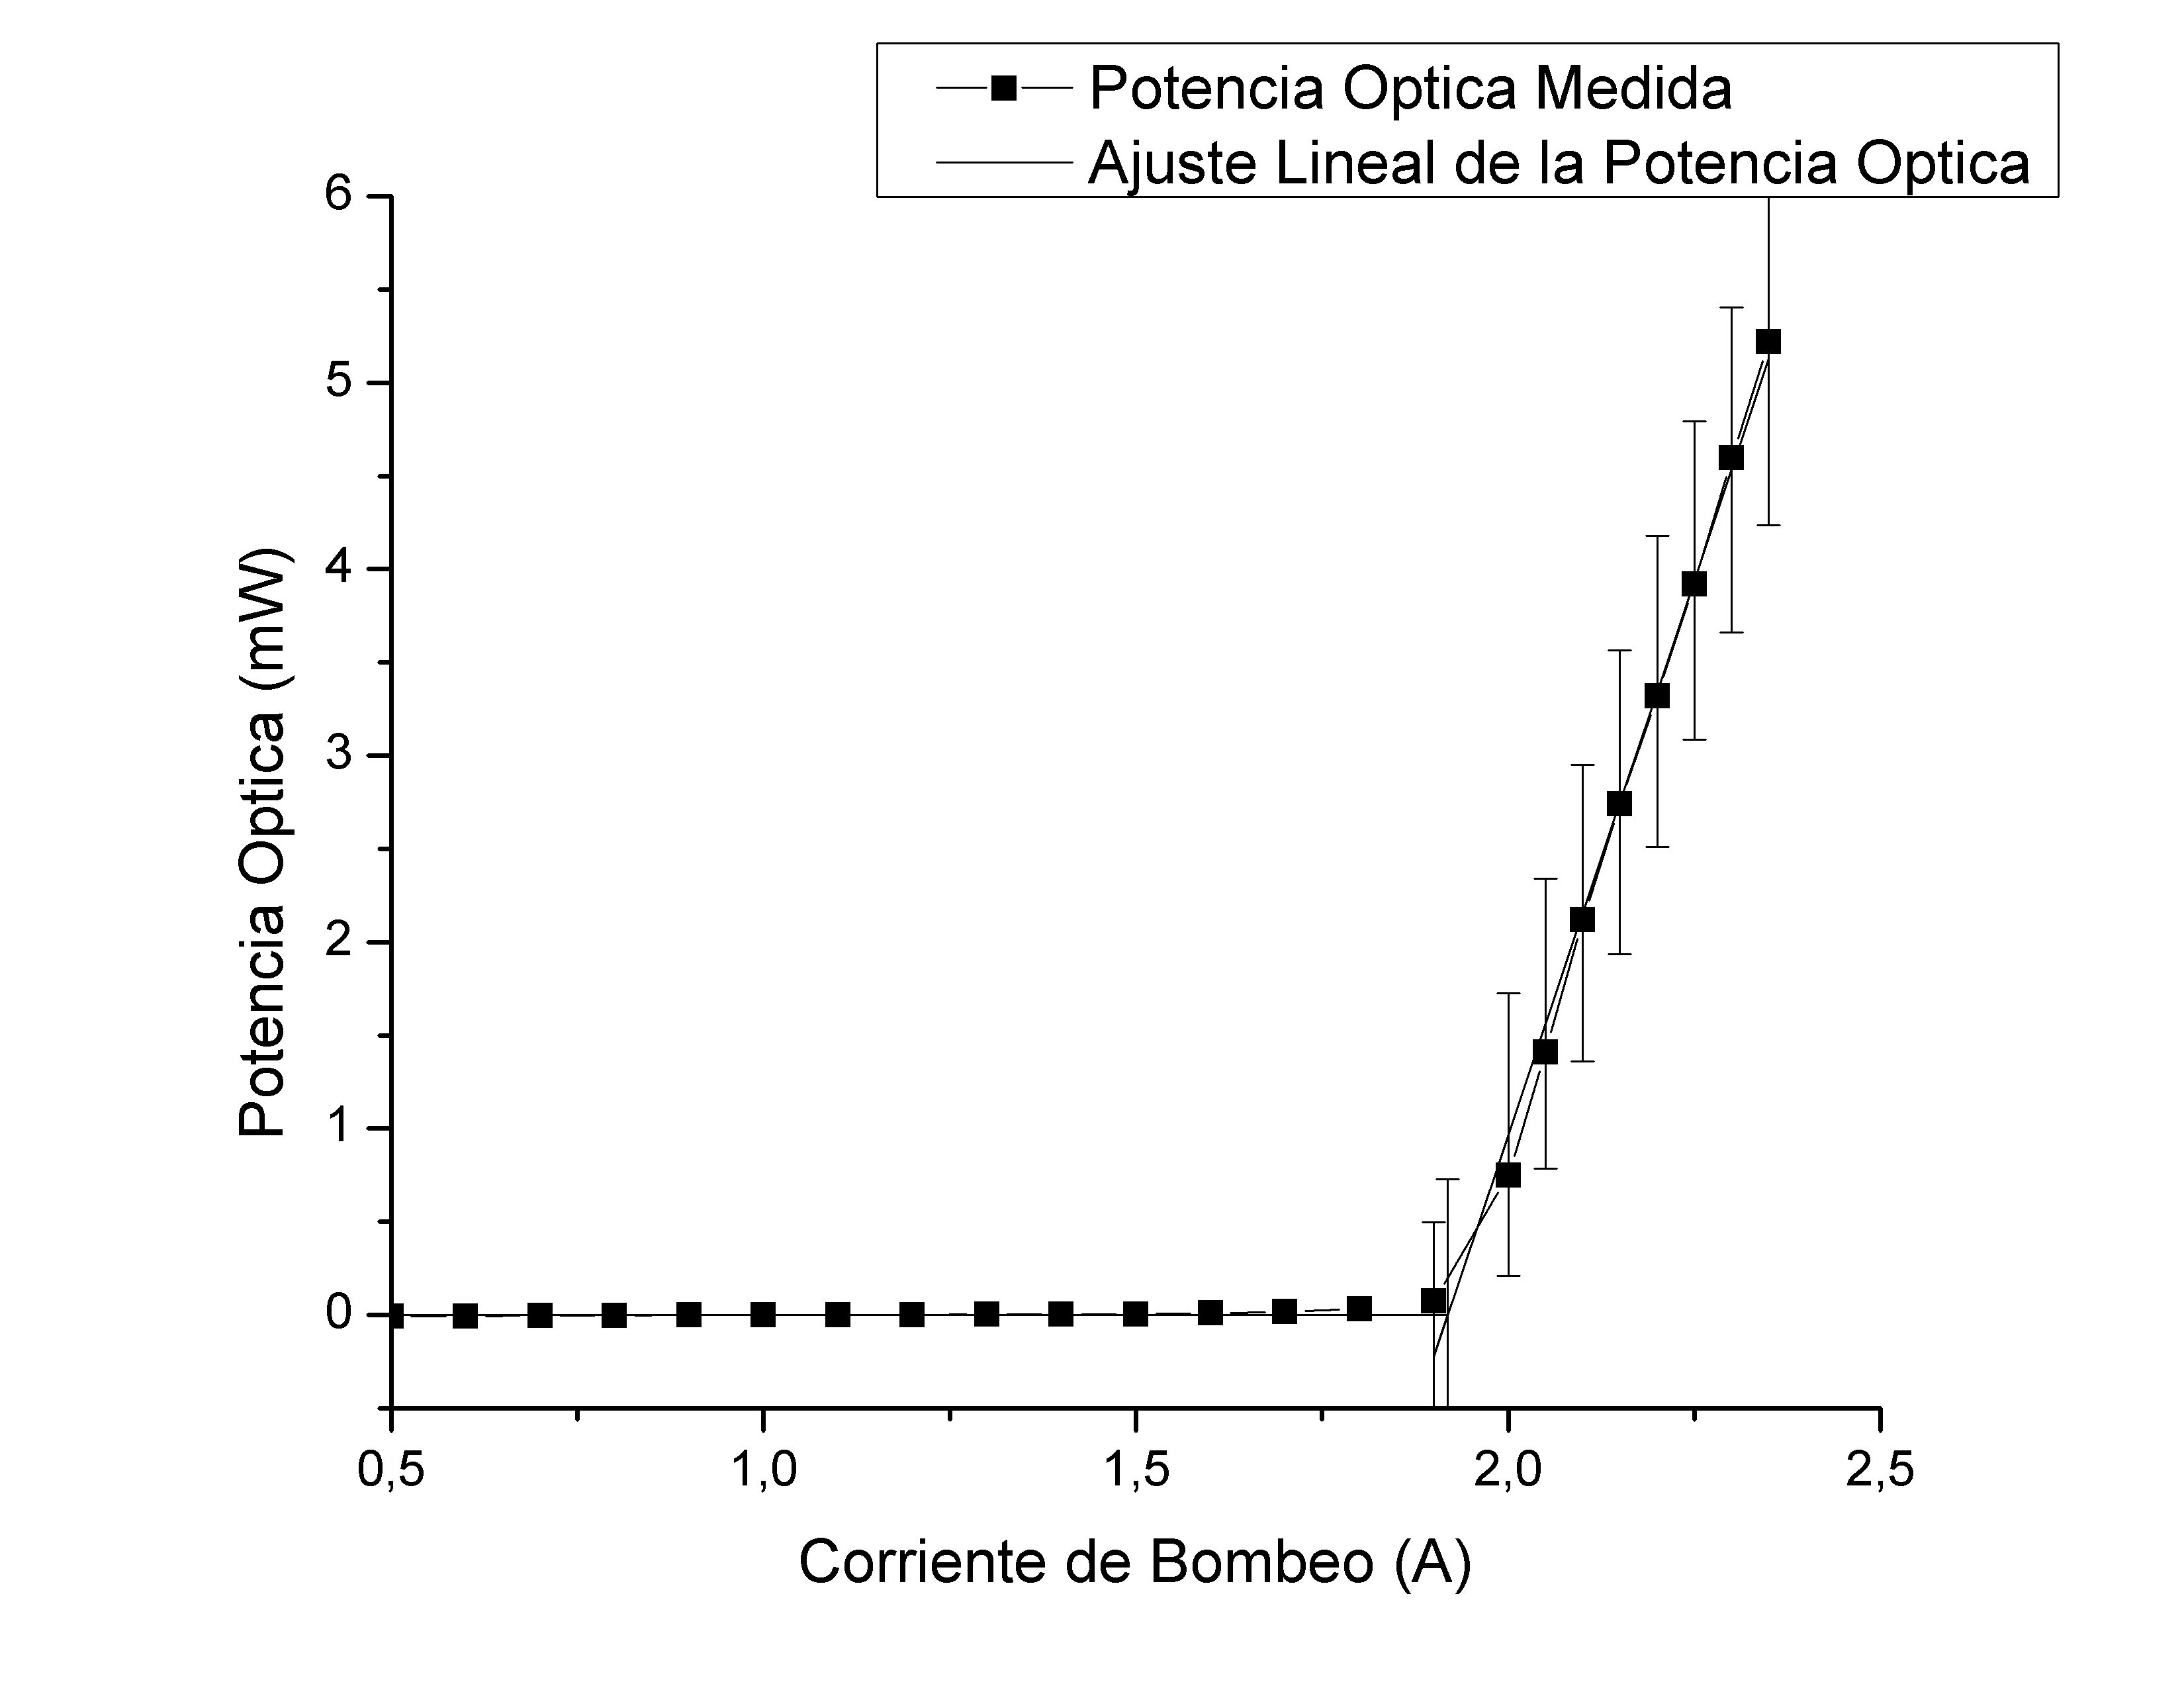
\includegraphics[scale=0.3]{Graficos/potlaservscorr.png}
    \caption{Potencia óptica de láser en función de la corriente de bombeo. La potencia aumenta linealmente a partir de 1.9A.}
    \label{laservscorr}
\end{figure}

\begin{figure}[H]
    \centering
    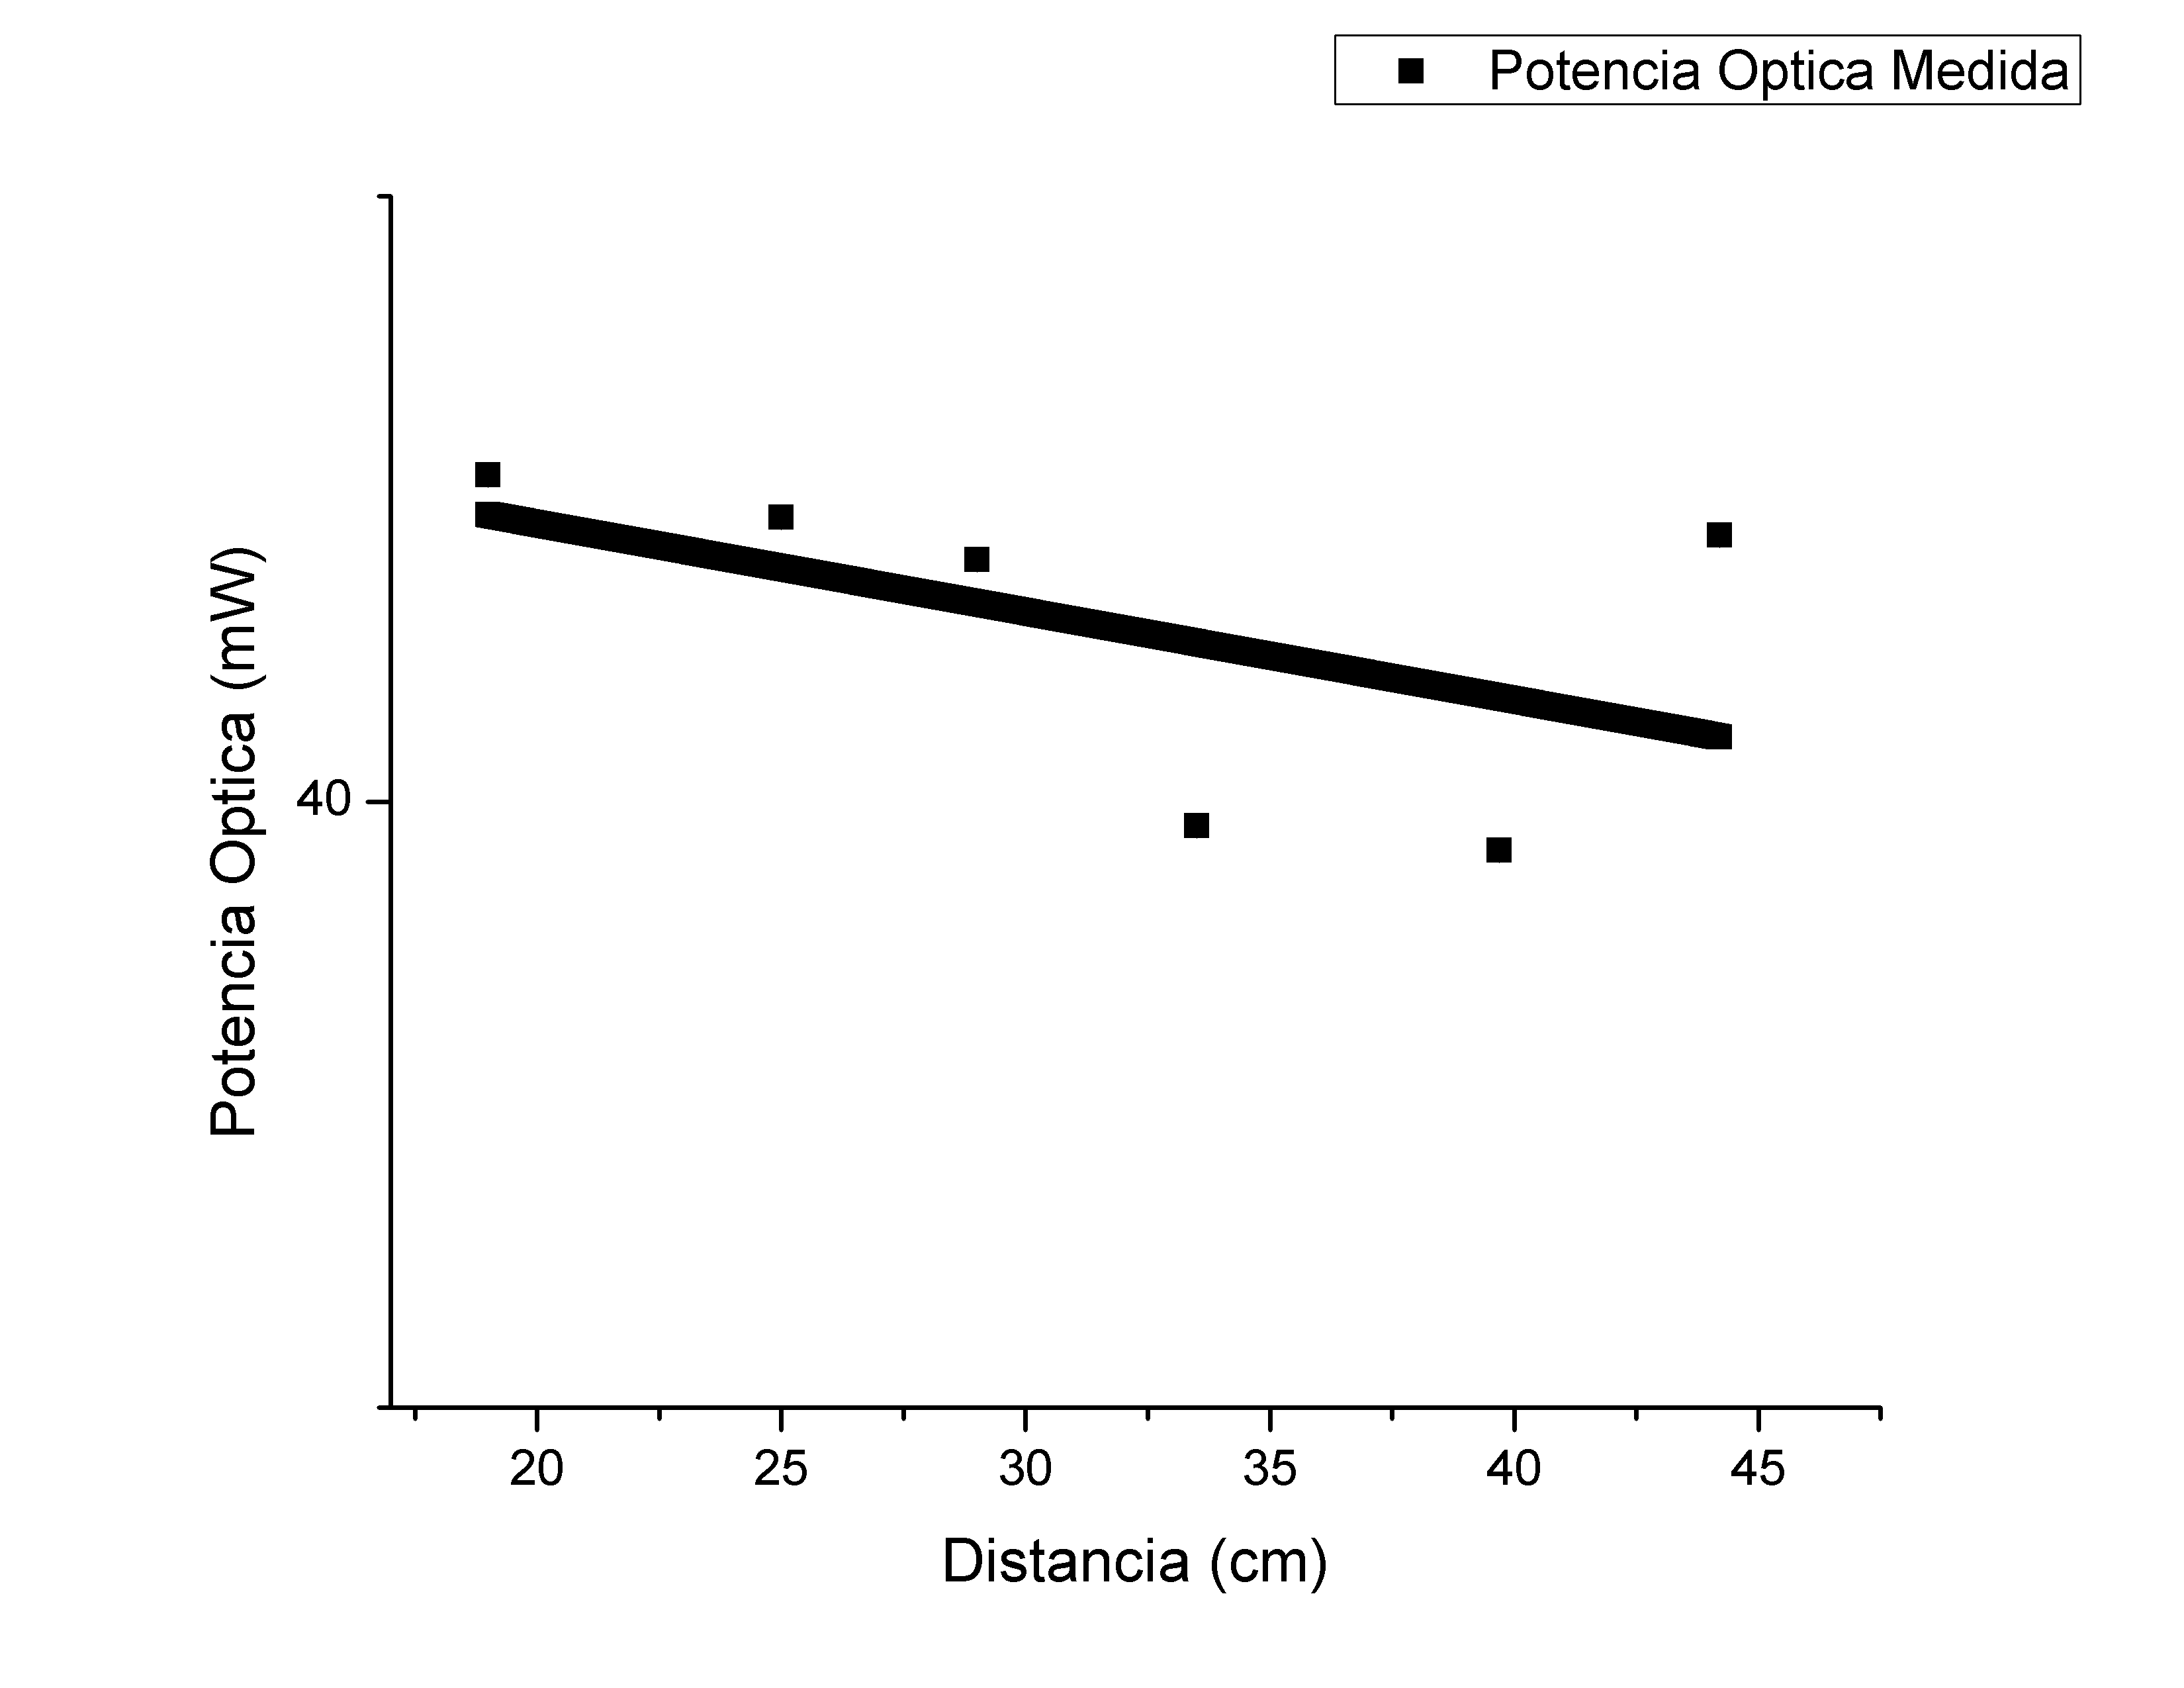
\includegraphics[scale=0.3]{Graficos/potlaservsdist.png}
    \caption{Potencia óptica de láser en función de la distancia para una corriente de bombeo constante de 2.39A.}
    \label{laservsdist}
\end{figure}

\begin{figure}[H]
    \centering
    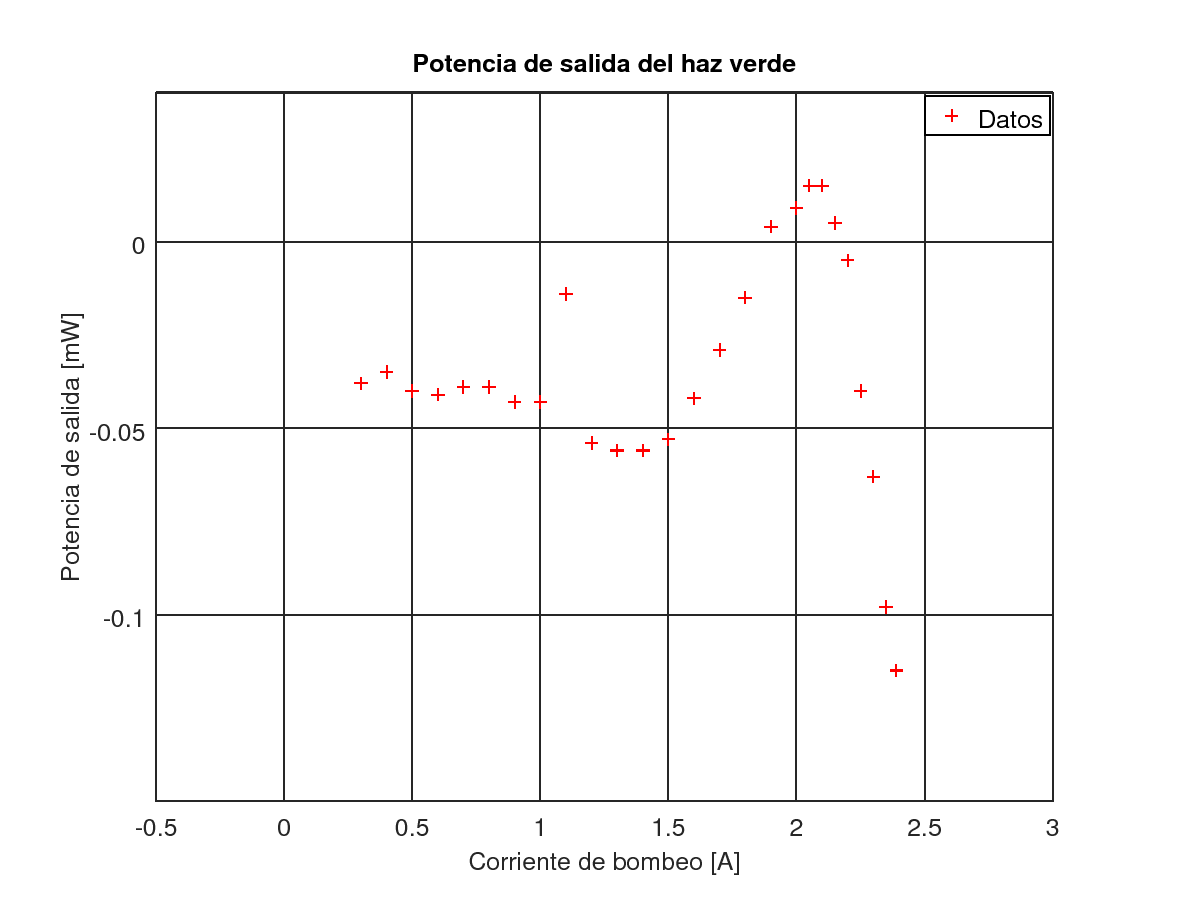
\includegraphics[scale=0.4]{Graficos/pot_verde.png}
    \caption{Potencia 2do armónico verde}
    \label{laservsdist}
\end{figure}

\begin{figure}[H]
    \centering
    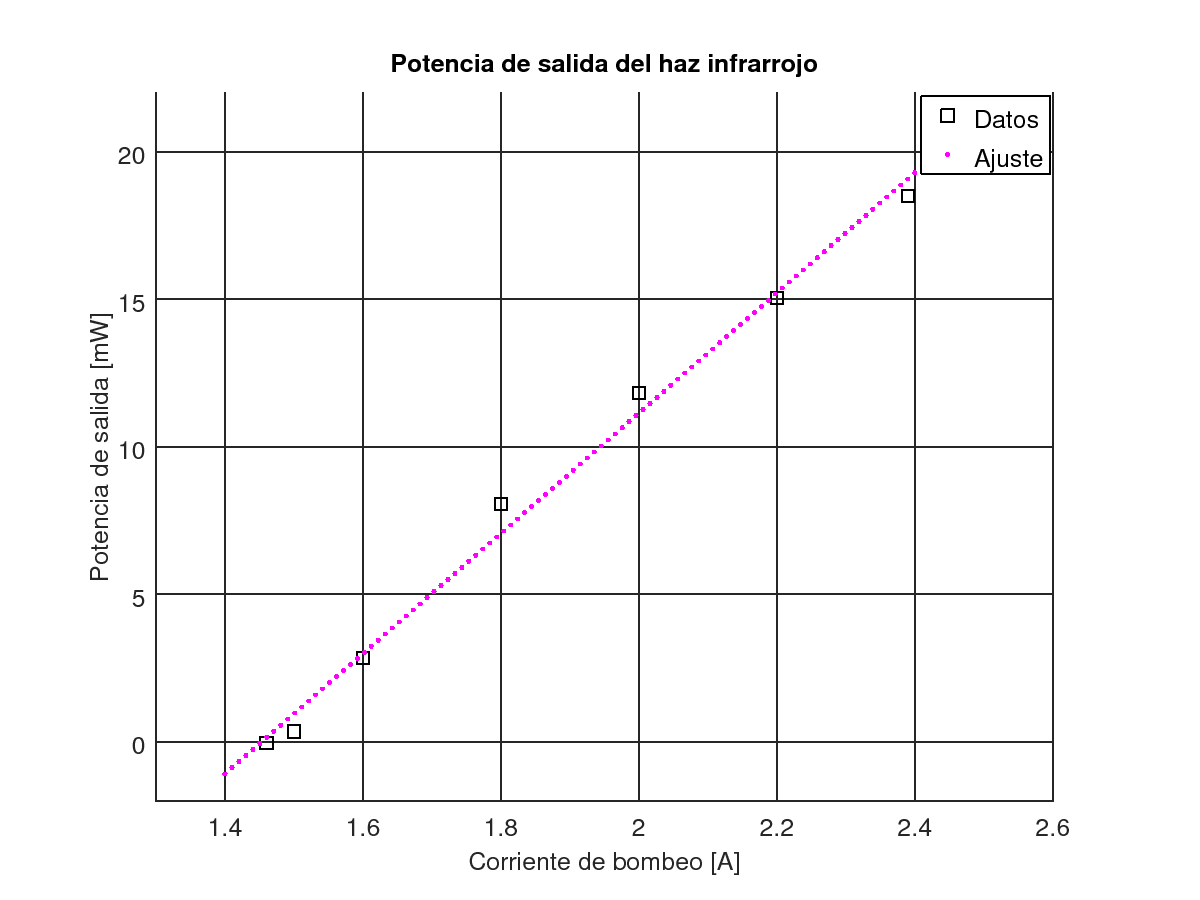
\includegraphics[scale=0.4]{Graficos/pot_infrarrojo.png}
    \caption{Potencia 2do armónico infrarrojo + ajuste lineal}
    \label{laservsdist}
\end{figure}



\section{Conclusiones}
% \addcontentsline{toc}{section}{Conclusiones} % Adds this section to the table of contents

%----------------------------------------------------------------------------------------
%	BIBLIOGRAPHY
%----------------------------------------------------------------------------------------


\begin{thebibliography}{100}
\bibitem{1}{Apuntes de la materia, \url{http://users.df.uba.ar/bragas/Labo5_1er2011/laser2k.pdf}}
\bibitem{2}{Robert W. Boyd, \textit{Nonlinear Optics}, 3ra edición, Academic Press, Inc, 2008.}
\end{thebibliography}
%----------------------------------------------------------------------------------------
\end{multicols}
\end{document}
